% CHAPTER 3 LESSON 1
\clearpage
\section{Fourier transformation (continuous time vs. discrete time)}
\label{Fourier transformation (continuous time vs. discrete time)}


%Einf�hrung in das Kapitel

Usually in signal processing, what we would like to do is modify a signal to some extent. For this it is important that the properties we want to modify are easily accessible. In the previous chapeter, we already saw that the fundamental period is an example of a speech property that is not so easily accesible in the time domain. It can be seen in the time domain, however it was shown that time domain based algorithms (ie.peak and zero crossing measurement) are prone to errors. It can then be beneficial to look at some transformation of the signal. Using the example of fundamental frequency estimation, it was shown that the autocorrelation function makes the estimation of the fundamental period more robust. A different concept is to look at the frequency content of signals. For instance, we have already seen some spectrograms of voiced speech. These produce a time/frequency based visualization that allows us to see the fluctuation of the spectral envelope.  It was shown that the spectral envelope is formed by the vocal tract and corresponds to the meaning of a sound and is what we use to distinguish between two phonemes. A narrow-band spectrogram can also reveal the fundamental frequency and its harmonics.  \\

This process of decomposing a signal into its frequency contents in order to make certain signal properties more accesible is known as Fourier theory. In Fourier analysis a signal is basically correlated with complex exponential functions, and because any exponential function can be written as a sum of cosine and sine functions, this means that it is correlated with cosine and sine functions. Because these exponentials can be shown to be linearly independent of each other(eigenfunctions), Fourier anaylsis preserves all of the original information and is therefore a completetly invertible function. This implies that no information is added or removed in the analysis and that it is simply a different way of representing the signal.  Certain attributes of the signal are made more visible whereas others are not visible any more. \\

 A pure tone is a tone that consists of only one sinusoid with a certain amplitude, frequency and phase. Note that this also includes a cosine function as a cosine is just a sine with a 90° phase shift. This pure tone is what we call a sinusoidal signal, and one of the key concepts of Fourier theory is that any periodic signal can always be represented as a sum of weighted sinusoids at the signals fundamental frequency and its harmonics, integer ultiples of the fundamental frequency. This is known as a Fourier series analysis.  Fourier theory can also be extended for arbitrary (non periodic) signals. The signal can then be shown to be composed of the integral over all frequencies that are in the signal, the spectrum of the signal.  This process is known as a Fourier analysis. \\

Figure 3.1 shows an example of a fourier series analysis of a rectangular function. The top sinusoid depicts the contribution of the fundamental period to the analysis. The second signal is the sum of the fundamental and a weighted third harmonic. It can be seen that the sum is a bit more close to the rectangular function, and as the number of harmonics is increased, a better approximation to original signal is achieved. The figure on the right shows how to weight the harmonics to get as close as possible to the square wave, and it can be seen that the majority of the energy is in the fundamental frequency with an exponential decay for the higher harmonics.  Another way of thinking about it is that at the edges of the rectangular function, there is a very sudden jump in the time domain, corresponding to a very high frequency content. Theoretically, one would need infinitely many harmonics to model the signal perfectly.\\

\begin{wrapfigure}{r}{0pt}
    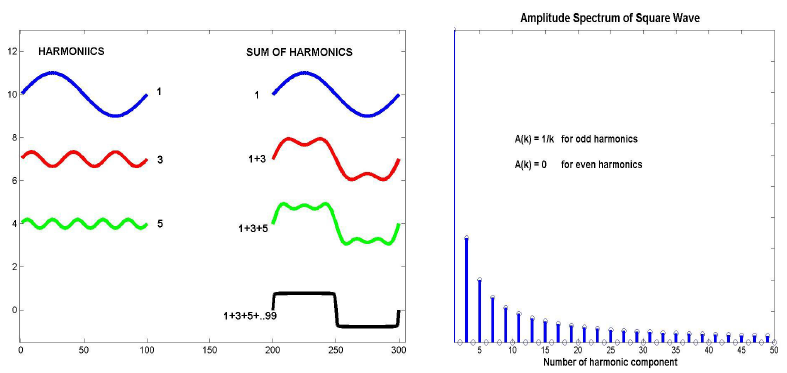
\includegraphics[width=0.7\textwidth]{Pictures/Chapter3_Lesson_1/FourierSquare.png}
    \caption{Fourier series analysis of a square wave.}
\end{wrapfigure}

Equation 3.1 is the mathematical representation of this process. The value, \begin{math}\cosCoef_0\end{math}, is called the DC offset and is the mean value about which the signal oscillates, in this case it is zero. The signal is therefore represented by this DC offset, and weigted contributions of sine and cosine functions at multiples of the fundamental frequency of the original signal. These weights are determined by correlating the original signal with cosine functions to determine the coefficients  \begin{math}\cosCoef_h\end{math} and sine functions to determine the coefficients \begin{math}\sinCoef_h\end{math}. Because the cosine function is an even function, whereas the rectangular function is odd, there will be zero correlation between the two. Therefore, the \begin{math}\cosCoef_h\end{math} coeffficients will all goto zero, leaving only the \begin{math}\sinCoef_h\end{math} coefficients to represent the signal. This can be seen in the right of Figure 1 along with the exponential decay of the weighting of the higher harmonics. \\

   \begin{tikzpicture}
\node [mybox] (box){%
    \begin{minipage}{0.50\textwidth}
    \begin{center}
    \begin{equation}x(t) = \frac{\cosCoef_0}{2}+\sum^{\infty}_{h=1}(\cosCoef_h\cos(2\pi hf_0t))+(\sinCoef_h\sin(2\pi 		hf_0t))
    \end{equation}
    \end{center}
  \end{minipage}
};
\node[fancytitle, right=10pt] at (box.north west) { Fourier series analysis};
\end{tikzpicture}%
  


Another reason why frequency analysis is a tool so often used in audio processing is that we also perceive sound in the frequency domain. This was introduced in the section on hearing regarding the frequency decomposition performed in the inner ear at different positions along the cochlea. This place coding implies that the cochlea performs a mechanical frequency analysis and that humans, in a sense, perceive sound in the frequency domain. This is the reason that it is quite natural for us to look at audio signals in the frequency domain. Computation can also be made much simpler in the spectral domain as convolution in the time domain corresponds to multiplcation in the frequency domain. This is often much easier to compute and is also another reason why spectral analysis can be the right tool to analyze certain signals.\\
  
  
  
%  
%  This is an example to get an idea of what frequency means what you can do is take a speech signal and filter out certain frequencioes andthen you get an idea of there certain contribuitions. SO this for instance is a speech signal with an audio bandwidth od 4khz. So if you throw away the frequencies higher than 2 khz we can stil understand but it doesnt sound nice anymore.  If we just look at the high frequency part, we only herar very little and it rather difficult to undertand and this is also because important formans are missing nowAnd if we just cut out frequencies between 500 and 1500Hz you can also get some odd distortions as opposed to the original.

  \begin{tikzpicture}
\node [mybox] (box){%
    \begin{minipage}{0.50\textwidth}
    \begin{center}
    \begin{equation*}
    X(\jmath\omega) = \int_{-\infty}^\infty x(t)e^{-\jmath \omega t} \mathrm{d}t
    \quad\quad\quad\quad x(t) = \frac{1}{2\pi} \int_{-\infty}^\infty X(\jmath \omega) e^{\jmath \omega t} \mathrm{d} \omega
    \end{equation*}
    \end{center}
  \end{minipage}
};
\node[fancytitle, right=10pt] at (box.north west) {Continuous-time Fourier transform};
\end{tikzpicture}%
   
    
  However, not all signals are periodic and eligible for Fourier series analysis.  In these cases, the continuous-time Fourier transform (Eq 3.2) can be used to represent any arbitrary signal. Any continuous time domain signal can be represented by a continuous frequency domain signal by bascially correlating the signal with complex exponentials over all frequencies, \begin{math}\omega\end{math}. And because complex exponentials can be represented with sines and cosines, this is like correlating the signal with sine and cosine functions over all frequencies, \begin{math}\omega\end{math}. In this sense, it is somewhat similar to the computation of the Fourier series coefficients, however the difference is that we now correlate over an infinite number of frequencies, not just the fundamental frequency and its harmonics.\\
  
   \begin{tikzpicture}
\node [mybox] (box){%
    \begin{minipage}{0.50\textwidth}
    \begin{center}
    \begin{equation*}
     X(e^{\jmath\omega}) = \sum_{\timei =-\infty}^\infty x(\timei ) e^{-\jmath \timei \omega}
      \quad\quad\quad\quad
      x(n) = \frac{1}{2\pi} \int_{-\pi}^\pi X(e^{\jmath\omega}) e^{\jmath\timei\omega}\mathrm{d} \omega
    \end{equation*}
    \end{center}
  \end{minipage}
};
\node[fancytitle, right=10pt] at (box.north west) {Discrete-time Fourier transform};
\end{tikzpicture}%
  
   
  
 The signals that we will be dealing with in digital speech processing will not be continuous, but discretized and sampled in the time domain.Therefore, we define the discrete time Fourier transform, DTFT. This is a transform with a discrete time index, \begin{math}\timei\end{math} but still a continuous frequency representation, \begin{math}\omega\end{math}. Here again,\begin{math}\omega\end{math} can take on an infinite number of values between 0 and \begin{math}2\pi\end{math}, wheras \begin{math}x(\timei)\end{math} is a finite,discrete representation of the original continuous signal. \\
  
    There are certain properties of the DTFT that can be related to the continuous time Fourier transform.  Looking at the definition of the DTFT in Eq2, we begin with the discrete time domain signal, \begin{math}x(\timei)\end{math}. To compute the frequency representation, instead of an integral, there is a summation.  The discrete time domain signal, \begin{math}x(\timei)\end{math} is  multiplied by phase shifted complex exponential functions and then summed. It is also important to note that, for the DTFT,  \begin{math}\timei\end{math} can only take on integer values. To return to the time domain, you would integrate over all frequencies again multiplied with these complex exponentials (conjugate?). Again these two transforrms are perfectly invertible meaning that there is no information lost upon conversion from time to frequency domain and vice versa.\\
    
 Because an integral and a summation are linear operators, the Fourier transform is itself linear. If you have a signal corresponding to the linear superpostion of two other signals, possibly even weighted with some scalar, then the Fourier transform of the sum of the two signals is equivalent to the sum of the Fourier transform of each signal. This is the basic defintiion of linearity and how we define a linear system. \\
  
 Very often in digital speech processing, we look at real valued signals in the time domain.  For example, a recording of an audio signal is real valued, implying that the spectrum is complex conjugate symmetric. This means that the real part is even while the imaginary part is odd. We can therefore also look at the even and the odd parts of the time domain signal separately. As introduced before, if  an even signal is correlated with a complex exponential, it is correalted with an even function, a cosine, and an odd function, a sine. The correlation between an even function and an odd will goto zero because of their opposing symmetries. When multiplied by the sine function, all values to the right of the origin will have equal, but opposing values, to the left of the origin, and the sum of the two will goto zero. \\
 
% So this means that the odd part of signal corresponds to the imaginary part of a spectrum.
% 
% Then a very basic property ist that the convolution, this is something you should all know.  A convolution in the time domain corresponds to a multiplecation in the frequency domain.
 
% Then a time shift, if you shift your signal in time, it corresponds to a taking the spectrum of a signal and modulating it with a omeag times the time shift.   It also goes the other way around if you shift your signal in the frequenccy domain, you have to modulate you signal in time domain. All of this properties are quite simple to derive.  All you have to do is the definitions of the FOurier transform and plug them in on one of the sides, and then you can derive all of these relations quite easy.  The last one is Parsevals theorem which also says the energy in a signal will be preserved when you take the Fourier analysis of a signal.


    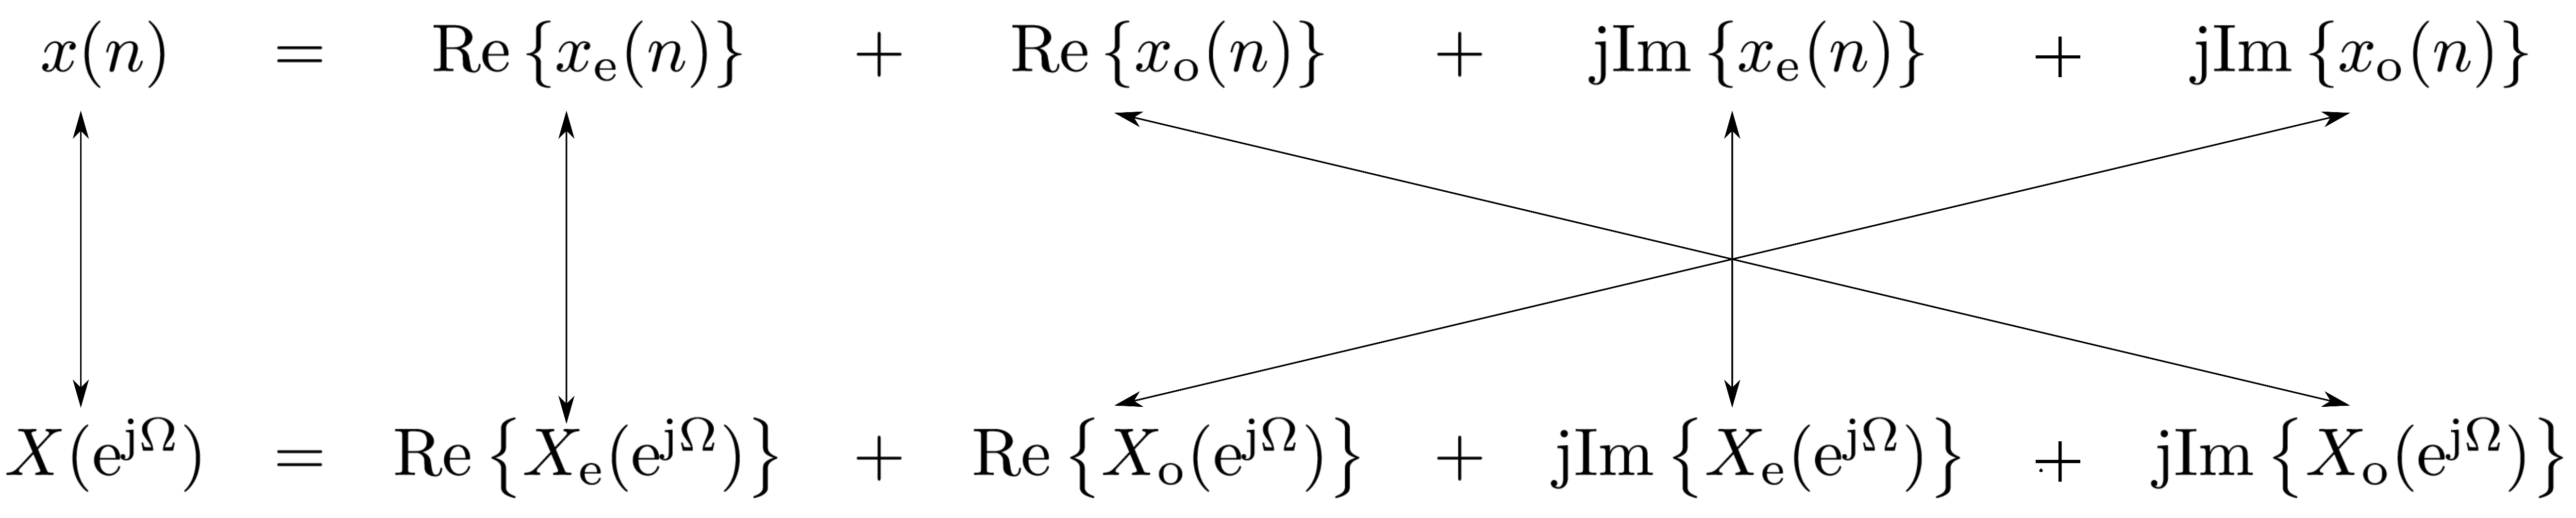
\includegraphics[width=0.7\textwidth]{Pictures/Chapter3_Lesson_1/dftSymmetry2-eps-converted-to.pdf}
   
 
 So, symmetry relations.  So this again relates to the analysis of the even and the odd part that I talked about before.  SO of coure, you can take a signal and it Fourier transform and you get the complex valued signal in the spectral domain . As we said, if you have areal valued and even signal, this corresponds to a real valued and even signal in the spectral domain.  However if real valued and odd signal, this corresponds to an imaginary and odd signal in the spectral domain. This is the representation that we will be working with most. Mostly we will be working with real valued signals meaning that you have a complex conjugate symmetric spectrum.  You could also make the same relations for complex signals then you would see that the the even paret of the imaginary part of a signal correposnds to the imaginary part of the spectrum, while the imaguinary parrtr and odd part corresponds to the reall value, but odd part of the specrtum.
 
 There are more relations in the spectral domain, and that is that whenever you have a discret time signal, this corresponds to a periodic spectrum and vice versa, if you have periodic signal, you would get a discrete spectrum. And when you kow this, you can do all  combinations of the two properties, for instance, if you have  continuous time signal that is not periodic. Also in the spectral domain, you would have a continuous spectrum that is not periodic. Then, if you have a continuos time signal that is periodic, for instance a vowel, you would have a discreter frequency and non periodic spectrum.  SO why when I have a vowel and lets say I do y frequency analysis why would I have a discrete frequency spectrum, or how would these discrete frequencies look.  The answer is that there are periodicites in the time domain signal corresponding to the fundamental period and its harmonics.  A frequency analysis of thi swould reveal discretized peaks in the spectral domain. So also if you have a discrete time signal, but also periodic at the same time, you would also have a discrete and periodic signal in the spectral domain and if you had a discrete signal that is not periodic, you would have a continous frequency spectrum, but periodic. So all of these four relations just stem from the two above. Here is a visualtization:
 
This is also important ot know, that if you have arectangular function, that in the fourier domain it corresponds to a synch function in the spectral domain.


